\documentclass[conference]{IEEEtran}
\usepackage{cite}
\usepackage{amsmath,amssymb,amsfonts}
\usepackage{graphicx}
\usepackage{textcomp}
\usepackage{xcolor}
\def\BibTeX{{\rm B\kern-.05em{\sc i\kern-.025em b}\kern-.08em
    T\kern-.1667em\lower.7ex\hbox{E}\kern-.125emX}}

\newcommand{\fl}{\mathrm{fl}_{32}}

\begin{document}

\title{Physics-Separable Hierarchical Compression of\\ 3-D Radar Power-Density Fields with\\ Pointwise Error Bounds and Random Access}

% Authors, affiliations and funding: to be provided by the authors.
\author{\IEEEauthorblockN{[Author names]}
\IEEEauthorblockA{\textit{[Department, organization]}\\
[City, country]\\
[e-mail]}
}

\maketitle

\begin{abstract}
Urban radar coverage studies produce simulated direct-path power-density fields on fine three-dimensional grids and read them through random point queries. Two features make such fields hard for general error-bounded compressors: adjacent nodes may straddle an occlusion boundary where the value drops to exactly zero, and outside the elevation scan window the nonzero values oscillate by orders of magnitude. We present the Physics-Separable Hierarchical Codec (PSHC), which stores a field as a propagation model identified from the data, a losslessly coded zero mask, and sparse multiplicative corrections. An octree selects the cheapest representation of each block, and a candidate is accepted only after the encoder reproduces the decoder's arithmetic and verifies the pointwise relative error bound at every node, so zeros are restored exactly. On loading, the file becomes a cell-indexed structure that answers a point query in constant time. On 20 fields (10 sites, two scan windows, $512^3$ nodes) and three error bounds, all 60 configurations meet the bound. Geometric-mean compression ratios are $1.15\times10^4$--$1.99\times10^4$, 11--77 times those of the best valid baseline (SZ3) for a $0^\circ$--$90^\circ$ window and $1.4\times10^3$--$1.8\times10^3$ times for a $30^\circ$--$60^\circ$ window. At a 0.1\% bound, latency-bound point queries are 4.1--9.5 times faster than reads of the raw array and throughput-bound queries at most 1.6 times slower.
\end{abstract}

\begin{IEEEkeywords}
error-bounded lossy compression, scientific data, radar coverage, context mixing, random access
\end{IEEEkeywords}

\section{Introduction}

Planning radar coverage in cities requires the power density a radar delivers to every point of a three-dimensional region, including the shadows cast by buildings~\cite{kostic2003radar,chen2008representation}. Such fields are computed by testing lines of sight against city models and are stored on regular grids~\cite{jiao2026vrpf}. At 1~m spacing a 1024~m cube holds $1.07\times10^9$ nodes, or 4.29~GB per radar configuration in single precision, and comparing sites or radar parameters multiplies this volume. Downstream simulations read the field through random point queries. A compressed representation must therefore bound the error at every node, decode without the generating program, and answer a query without decompressing the field.

Fig.~\ref{fig:method}(a) shows why these fields resist general-purpose compression. Neighboring nodes often straddle an occlusion boundary, where the value falls from a smooth level to exactly zero. Outside the elevation range swept by the beam, the nonzero values follow the side lobes of the antenna pattern and change by orders of magnitude between vertically adjacent nodes. Error-bounded lossy compressors such as SZ3~\cite{liang2023sz3}, ZFP~\cite{lindstrom2014zfp} and SPERR~\cite{li2023sperr} exploit local smoothness through prediction or transforms, which both features break. Their native error bounds are absolute or relative to the value range, so a pointwise relative bound requires a logarithmic transform~\cite{liang2018pwr,zou2019msst} and a separate treatment of zeros, and answering a point query generally means decompressing a block or the whole array. Sparse volume structures such as VDB~\cite{museth2013vdb} and NanoVDB~\cite{museth2021nanovdb} give fast random access but gain little here, because much of the urban space is visible and the field is not sparse.

Both difficulties come from the physics that generates the data. Apart from occlusion, a value is a smooth point-source decay multiplied by an antenna pattern factor that depends only on elevation, and both are described by a few parameters. If the decoder can evaluate these factors, a field is described mainly by where its zeros lie, plus small local deviations. This paper builds on that observation with the following contributions:
\begin{itemize}
\item a physics-separable, self-contained representation: a parametric model identified from the data alone, a losslessly coded zero mask, and sparse multiplicative corrections (Sections~\ref{sec:repr}--\ref{sec:ident});
\item pointwise error control by construction: an octree chooses the representation of each block by estimated code length, and every candidate is verified against the original error condition with the decoder's own arithmetic, with a raw fallback (Section~\ref{sec:tree});
\item a query structure that expands the file into fixed-size cells and answers a point query with a constant number of memory accesses (Section~\ref{sec:query});
\item an evaluation on 60 configurations against SZ3, ZFP, SPERR and SZ2 under the same pointwise error contract (Section~\ref{sec:exp}).
\end{itemize}

\begin{figure*}[t]
\centering
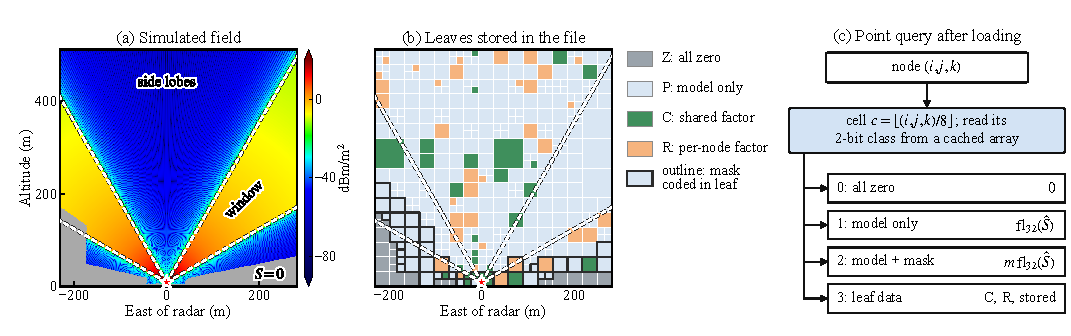
\includegraphics[width=\textwidth]{figs/fig_method.pdf}
\caption{PSHC on the east--west vertical section through the radar at site P03 ($30^\circ$--$60^\circ$ window, $\varepsilon=0.1\%$). (a)~Original field in dBm/m$^2$; grey nodes are occluded ($S=0$), dashed lines mark the window edges and the star marks the radar. (b)~Octree leaves of the 40.7~kB compressed file on the same section: open sky becomes large model-only leaves, buildings become zero leaves, and small leaves gather along occlusion boundaries and near pattern nulls. (c)~Point query on the loaded structure; $m$ is the node's mask bit and $\hat S$ the model value.}
\label{fig:method}
\end{figure*}

\section{Problem and Representation}\label{sec:repr}

\subsection{Input and Error Contract}

The input is a nonnegative single-precision field $S(i,j,k)$ in W/m$^2$ on a regular grid of nodes $(i,j,k)$ with 1~m spacing; $S$ is zero at nodes not visible from the radar. Given an error bound $\varepsilon>0$, the decoded field $\tilde S$ must satisfy
\begin{equation}
|\tilde S(i,j,k)-S(i,j,k)|\le\varepsilon\,S(i,j,k)
\label{eq:contract}
\end{equation}
at every node. Condition~\eqref{eq:contract} is a strict per-node requirement rather than an average; at $S=0$ it forces $\tilde S=0$, so zeros must be restored exactly. Decoding must be self-contained: it may read only the compressed file, not the radar parameters or the generating program. Within these constraints we minimize the file size.

\subsection{Physical Structure of the Field}

The fields used here were generated with the VRPF framework~\cite{jiao2026vrpf}, which tests the line of sight from the antenna to every node against a photogrammetric city mesh and evaluates a far-field radar equation. Without atmospheric loss, the generator computes
\begin{equation}
S=V\,\frac{K\,G(\phi)}{R^2},\qquad K=\frac{P_tG_{\max}}{4\pi},
\label{eq:field}
\end{equation}
where $V\in\{0,1\}$ is the visibility, $R$ the distance and $\phi$ the elevation of the node seen from the antenna, $P_t$ the transmit power, $G_{\max}$ the peak gain, and $G$ the normalized pattern factor. The beam scans $360^\circ$ in azimuth and the elevation window $[\phi_1,\phi_2]$. A node inside the window meets the beam peak during the scan, so $G=1$. Outside, $G=F^2(s)$ with $s=\sin\delta$, where $\delta$ is the angular distance to the nearest window edge and
\begin{equation}
F(s)=\frac{\sin(As)}{N\sin(\beta s)},\qquad \beta=\frac{\pi d}{\lambda},\quad A=N\beta,
\label{eq:af}
\end{equation}
is the array factor of $N$ elements spaced $d$ apart at wavelength $\lambda$. Equations~\eqref{eq:field} and~\eqref{eq:af} define how the data were generated; the encoder does not know their parameters and identifies them from the data (Section~\ref{sec:ident}).

\subsection{Physics-Separable Representation}

Following~\eqref{eq:field}, PSHC writes the decoded value as
\begin{equation}
\tilde S=M\cdot\fl\big(\hat S\,\Phi\big),
\label{eq:repr}
\end{equation}
where $\fl$ denotes rounding to single precision. The zero mask $M$ equals 1 exactly where $S\neq0$. It coincides with $V$ except at visible nodes where $G$ vanishes, such as pattern nulls. The model prediction $\hat S$ is computed from parameters stored in the file, and $\Phi$ is a local multiplicative correction: $\Phi=1$ where the model is accurate enough, otherwise a factor shared by a block or one factor per node. Blocks for which corrections cost more than raw values store $S$ directly. Fig.~\ref{fig:method}(b) shows how these choices are distributed in a real file.

\section{Identifying the Model from the Data}\label{sec:ident}

For an isotropic point source, $1/S=R^2/K$ is a quadratic polynomial of the node coordinates. PSHC therefore models the envelope as
\begin{equation}
1/\hat S_0=a_1X^2+a_2Y^2+a_3Z^2+a_4X+a_5Y+a_6Z+a_7,
\label{eq:env}
\end{equation}
with coordinates $(X,Y,Z)$ centered on the grid. Equation~\eqref{eq:env} is linear in $a_1,\dots,a_7$, which are fitted by least squares on the relative deviations of sampled nonzero nodes while samples far from the current fit are iteratively rejected. The coefficients encode the equivalent source position, e.g., $Z_0=-a_6/(2a_3)$, so the radar location is recovered from the data.

The scan window and the pattern follow from the same samples. Because $G\le1$, unoccluded samples inside the window lie on the envelope and side-lobe samples fall below it, so $\rho=\ln(S/\hat S_0)\approx\ln G$. The elevation interval in which the samples cling to the envelope gives the window. The main-lobe roll-off just outside each edge gives $A$ and the edge position, and deeper side lobes give $\beta$. The resulting model is $\hat S=\hat S_0$ inside the window and $\hat S=\hat S_0F^2(s)$ outside it. Because the side-lobe phase $As$ amplifies elevation errors by a factor of about $A$ ($A\approx386$ for the radar of Section~\ref{sec:exp}), the envelope and the elevation outside the window are taken from a slightly richer polynomial geometry fitted to in-window samples. The parameters are refined to minimize the mean truncated log deviation $\frac1n\sum_n\min(|\ln(S_n/\hat S_n)|,1)$ over the $n$ samples. The pattern is kept only if it reduces the deviation; otherwise a simpler model is used. All parameters, a few hundred bytes, are stored in the file, so the decoder evaluates $\hat S$ at any node without the radar parameters. Identification affects only the file size; the error bound is enforced separately (Section~\ref{sec:tree}).

\section{Hierarchical Representation with Acceptance}\label{sec:tree}

\subsection{Log-Domain Corrections}

For $S>0$, condition~\eqref{eq:contract} is equivalent to $\ln(1-\varepsilon)\le\ln(\tilde S/S)\le\ln(1+\varepsilon)$. Because $|\ln(1-\varepsilon)|>\ln(1+\varepsilon)$, the symmetric condition
\begin{equation}
|\ln\tilde S-\ln S|\le d,\qquad d=\ln(1+\varepsilon),
\label{eq:logtol}
\end{equation}
is sufficient for~\eqref{eq:contract}. A per-node correction stores the integer $q=\mathrm{round}(\ln(S/\hat S)/\Delta)$ and decodes
\begin{equation}
\tilde S=\fl\big(\hat S\,e^{q\Delta}\big).
\label{eq:quant}
\end{equation}
Rounding $q$ contributes at most $\Delta/2$ to the log error and the floating-point evaluation a small $\eta$, so~\eqref{eq:logtol} holds whenever $\Delta/2+|\eta|_{\max}\le d$; PSHC sets $\Delta$ slightly below $2d$. In the log domain one step size serves values that span many orders of magnitude, whereas additive corrections would need a step proportional to each value. When the deviations $\ln(S/\hat S)$ of a block fall within a narrow range, one shared integer replaces the per-node ones.

\subsection{Leaf States and Acceptance}

Each octree leaf takes one of five states: Z (all zero), P (model only, $\Phi=1$), C (one shared factor), R (per-node factors), or RAW (raw values). P, C and R leaves that contain zeros are called mixed and also carry a coded zero mask. For a candidate state, the encoder reconstructs every node exactly as the decoder will, with the same single-precision operations, deterministic elementary functions and no fused multiply--add, and tests the original condition~\eqref{eq:contract} at every node. States are tried in order of increasing cost and the first that passes is kept; an R candidate may move $q$ by $\pm1$, and RAW always passes. Hence every decoded node satisfies~\eqref{eq:contract} by construction, whatever the accuracy of the model, and~\eqref{eq:logtol} serves only to choose $\Delta$.

\subsection{Octree Selection}

Leaves range from $512^3$ down to $8^3$ nodes. For a block $v$, the encoder compares the estimated code length of keeping $v$ as one leaf with that of splitting it,
\begin{equation}
C(v)=\min\Big(C_{\mathrm{leaf}}(v),\ b+\sum_{u\in\mathrm{child}(v)}C(u)\Big),
\label{eq:cost}
\end{equation}
where $C_{\mathrm{leaf}}(v)$ is the cost of the cheapest feasible state of $v$, $b$ the cost of a split flag, and $C(v)=C_{\mathrm{leaf}}(v)$ for $8^3$ blocks. The estimates count directory symbols, mask bits predicted by a dry run of the mask coder, and correction bits, and~\eqref{eq:cost} is evaluated bottom-up from statistics of $8^3$ cells. Leaves with a mask or per-node data are at most $32^3$, so each lies inside one $128^3$ superblock. Estimation errors affect only the size, because the final states are decided by acceptance. The tree and the state of each leaf form the leaf directory of the file.

\section{Entropy Coding and Point Queries}\label{sec:query}

\subsection{Coding}

Only mixed leaves need their zero mask coded; for all other leaves the directory or the raw values determine the zeros. The mask is coded per $128^3$ superblock, so superblocks can be decoded independently and in parallel. Nodes are visited in raster order across leaf boundaries. Five context models predict each mask bit from causal neighbors in the current and the two lower layers, from the number of unknown face neighbors, and from the distance to the source. Their predictions are combined by logistic mixing~\cite{mahoney2005mixing} and refined by two adaptive probability maps before arithmetic coding. All probability computations use integer arithmetic, so the encoder and the decoder stay bit-identical. In R leaves, $q$ is predicted from already coded neighbors with the best of six predictors per leaf, and the residuals are entropy coded.

\subsection{Query Structure}

On loading, the file is expanded into a flat structure over cells of $8^3$ nodes. Each cell lies in exactly one leaf and stores a 2-bit class and a directory entry; masks, shared factors, corrections and pre-decoded values reside in separate pools. A query for node $(i,j,k)$ reads the class of its cell (Fig.~\ref{fig:method}(c)). Class 0 returns zero, class 1 returns $\fl(\hat S)$, class 2 returns $m\,\fl(\hat S)$ with the node's mask bit $m$, and class 3 follows the entry to the leaf's shared factor, per-node correction or stored value. The class array takes 2 bits per cell, 64~KiB for a $512^3$ grid, and stays in cache, whereas random reads of a raw 512~MiB array mostly miss it. Cells whose model values involve the pattern are pre-decoded if this needs at most 64~MiB; otherwise the pattern is evaluated at query time, and such cells with a shared factor or only a few non-model values also use classes 1 and 2. Either way, a query returns exactly the value of full decoding. We report three costs separately: the file on disk, the memory of the loaded structure, and the time per query after loading.

\section{Experiments}\label{sec:exp}

\subsection{Data and Protocol}

The fields were generated with VRPF~\cite{jiao2026vrpf} for a 500~m$\,\times\,$500~m urban area. A vehicle-mounted radar with its antenna 3~m above the street was placed at ten sites (P01--P10) and simulated with two elevation windows, $0^\circ$--$90^\circ$ and $30^\circ$--$60^\circ$. The radar has $N=256$ elements with $d/\lambda=0.48$ at 24~GHz, a 25~dB peak gain and 1~W transmit power. Each field has $512^3$ nodes at 1~m spacing (512~MiB), of which 8.5\%--83.6\% are nonzero. With $\varepsilon\in\{1\%,0.1\%,0.01\%\}$ this gives 60 configurations. All runs used one computer with an Intel Core i7-14650HX, 8 logical CPUs and 32~GB of memory.

The baselines are SZ3 3.4.0~\cite{liang2023sz3}, ZFP 1.0.1~\cite{lindstrom2014zfp} and SPERR 0.8.5~\cite{li2023sperr}. None supports a pointwise relative bound, so we apply the usual logarithmic transform~\cite{liang2018pwr} with the bound converted to the log domain. Zeros are handled either by SZ2's sentinel value or by a separately stored zstd~\cite{collet2021zstd} bitmap, with zero positions filled by a neighboring nonzero value, a constant, or push--pull interpolation~\cite{gortler1996lumigraph}. ZFP is also run with its bound enlarged 2 to 16 times, because its actual error often stays far below the requested bound. The two pointwise-relative modes built into SZ2~\cite{liang2018pwr,zou2019msst} complete 18 candidates per configuration. Every decompressed candidate is checked at every node, in double precision, by two independently written programs, and for each method the smallest valid file is kept, counting bitmaps and restoration parameters. On four fields, our baseline calls reproduced the output of the official command-line tools bit for bit. The compression ratio is the raw size divided by the compressed size, averaged geometrically over the sites. PSHC sizes include an optional per-leaf summary (5.6\%--9.8\% of a file at $\varepsilon=0.1\%$) that decoding does not use; the ablation excludes it.

\subsection{Compression and Validity}

\begin{table}[t]
\caption{Geometric-mean compression ratio over ten sites. Ratio: SZ3 file size divided by PSHC file size.}
\label{tab:cr}
\centering
\begin{tabular}{ccrrr}
\hline
Window & $\varepsilon$ & PSHC & SZ3 & Ratio\\
\hline
 & 1\% & 19\,903 & 1\,760.7 & 11.3\\
$0^\circ$--$90^\circ$ & 0.1\% & 19\,893 & 764.4 & 26.0\\
 & 0.01\% & 19\,851 & 258.6 & 76.8\\
\hline
 & 1\% & 19\,453 & 14.0 & 1\,391\\
$30^\circ$--$60^\circ$ & 0.1\% & 17\,604 & 9.8 & 1\,804\\
 & 0.01\% & 11\,534 & 7.4 & 1\,558\\
\hline
\end{tabular}
\end{table}

All 60 PSHC configurations satisfy~\eqref{eq:contract} at every node, with all zeros restored exactly. SZ3 is the best valid baseline in every configuration; Table~\ref{tab:cr} compares the two. The windows differ in what a baseline must encode. With the $0^\circ$--$90^\circ$ window almost all nonzero nodes lie inside the window and form a smooth point-source decay, which prediction handles well, yet every value must still be coded within the bound, so the SZ3 file grows as $\varepsilon$ shrinks. PSHC predicts these values, and about 90\% of its file is the zero mask, which does not depend on $\varepsilon$; the ratio therefore rises from 11.3 to 76.8. With the $30^\circ$--$60^\circ$ window more than 40\% of the nonzero nodes lie in the side lobes. Their oscillation defeats prediction and transforms, so the baseline files consist almost entirely of value streams, while PSHC predicts the side lobes from the pattern model and stays about three orders of magnitude smaller. At $\varepsilon=0.01\%$ more nodes near pattern nulls need corrections, which then make up a third of the PSHC file.

\subsection{Source of the Gain}

Disabling the pattern model shows where the gain comes from. For sites P03 and P08 with the $30^\circ$--$60^\circ$ window at $\varepsilon=0.1\%$, keeping only the point-source envelope makes the files 1\,721 and 2\,344 times larger than with the full method (sizes without the optional summary). Without the pattern, almost every side-lobe value deviates from the envelope by far more than the tolerance and must be stored as a per-node correction or a raw value.

\subsection{Point Queries}

Queries were timed on one thread after loading, with two access patterns. Independent queries visit $4\times10^6$ uniformly random nodes and overlap in the processor, which measures throughput; in dependent queries the next node is derived from the previous result, which measures latency. Both were compared with reads of the raw 512~MiB array in the same run; we report the median per query over five rounds and then the median over the ten sites. With the $30^\circ$--$60^\circ$ window at $\varepsilon=0.1\%$, an independent query takes 12.3~ns against 7.8~ns for the raw array, and a dependent query 25.0~ns against 102.8~ns. The loaded structure occupies 4.2~MiB, compared with about 30~kB on disk (geometric mean) and 512~MiB raw, and loads in 0.26~s with eight threads. Staying in cache shortens dependent queries. Independent queries are slower because at nine of the ten sites pre-decoding the side-lobe cells would exceed the 64~MiB budget, so the pattern is evaluated at query time. With the $0^\circ$--$90^\circ$ window both are faster than the raw array (3.6 vs.\ 7.7~ns and 10.8 vs.\ 102.1~ns) with a 2.9~MiB structure.

\subsection{Limits}

The compression gain presupposes that the field follows the model to within about the error bound. We multiplied the fields of P03 and P08 node by node by independent factors $e^{\xi}$, $\xi\sim\mathcal N(0,\sigma^2)$, with $\sigma=\varepsilon=0.1\%$. The two-site geometric-mean compression ratio then drops to 32.6 and 32.5 for the two windows, because nearly every leaf contains nodes outside the tolerance, yet all derived fields still satisfy~\eqref{eq:contract} at every node. Model fit thus governs the compression gain, while pointwise acceptance alone guarantees the accuracy. These conclusions are limited to the simulated direct-path fields and configurations tested.

\section{Conclusion}

PSHC compresses simulated radar power-density fields by separating what physics predicts from what geometry decides: a self-contained parametric model gives the values, a context-mixed mask gives the zeros, and sparse multiplicative corrections absorb the remainder. Acceptance with the decoder's own arithmetic makes the pointwise relative bound hold at every node, and a cell-indexed structure answers point queries in constant time. On 60 configurations PSHC met the bound everywhere and reached geometric-mean compression ratios of $1.15\times10^4$--$1.99\times10^4$, 11 to 1\,804 times those of SZ3. Its gain depends on how closely a field follows the model; measured antenna patterns and fields of several radars are left for future work.

\begin{thebibliography}{00}
\bibitem{kostic2003radar} A. Kostic and D. Rancic, ``Radar coverage analysis in virtual GIS environment,'' in \textit{Proc. 6th Int. Conf. Telecommun. Modern Satellite, Cable Broadcast. Service (TELSIKS)}, 2003, vol.~2, pp.~721--724.
\bibitem{chen2008representation} P. Chen and L. Wu, ``3D representation of radar coverage in complicated environment,'' \textit{Simul. Model. Pract. Theory}, vol.~16, pp.~1190--1199, 2008.
\bibitem{jiao2026vrpf} L. Jiao, A. Yang, Q. Jia, M. Ma, Y. Zhang, L. Wang, and J. Li, ``VRPF: A fine-grained 3D radar power-density computation framework based on photogrammetric city models for urban observation,'' \textit{Remote Sens.}, vol.~18, no.~12, Art. no.~1936, 2026, doi: 10.3390/rs18121936.
\bibitem{liang2023sz3} X. Liang \textit{et al.}, ``SZ3: A modular framework for composing prediction-based error-bounded lossy compressors,'' \textit{IEEE Trans. Big Data}, vol.~9, no.~2, pp.~485--498, 2023.
\bibitem{lindstrom2014zfp} P. Lindstrom, ``Fixed-rate compressed floating-point arrays,'' \textit{IEEE Trans. Vis. Comput. Graphics}, vol.~20, no.~12, pp.~2674--2683, 2014.
\bibitem{li2023sperr} S. Li, P. Lindstrom, and J. Clyne, ``Lossy scientific data compression with SPERR,'' in \textit{Proc. IEEE Int. Parallel Distrib. Process. Symp. (IPDPS)}, 2023, pp.~1007--1017.
\bibitem{liang2018pwr} X. Liang, S. Di, D. Tao, Z. Chen, and F. Cappello, ``An efficient transformation scheme for lossy data compression with point-wise relative error bound,'' in \textit{Proc. IEEE Int. Conf. Cluster Comput. (CLUSTER)}, 2018, pp.~179--189.
\bibitem{zou2019msst} X. Zou \textit{et al.}, ``Accelerating relative-error bounded lossy compression for HPC datasets with precomputation-based mechanisms,'' in \textit{Proc. 35th Symp. Mass Storage Syst. Technol. (MSST)}, 2019, pp.~65--78.
\bibitem{museth2013vdb} K. Museth, ``VDB: High-resolution sparse volumes with dynamic topology,'' \textit{ACM Trans. Graph.}, vol.~32, no.~3, pp.~27:1--27:22, 2013.
\bibitem{museth2021nanovdb} K. Museth, ``NanoVDB: A GPU-friendly and portable VDB data structure for real-time rendering and simulation,'' in \textit{ACM SIGGRAPH Talks}, 2021, pp.~1--2.
\bibitem{mahoney2005mixing} M. V. Mahoney, ``Adaptive weighing of context models for lossless data compression,'' Florida Inst. Technol., Melbourne, FL, USA, Tech. Rep. CS-2005-16, 2005.
\bibitem{collet2021zstd} Y. Collet and M. Kucherawy, ``Zstandard compression and the `application/zstd' media type,'' RFC 8878, Internet Engineering Task Force, 2021.
\bibitem{gortler1996lumigraph} S. J. Gortler, R. Grzeszczuk, R. Szeliski, and M. F. Cohen, ``The lumigraph,'' in \textit{Proc. 23rd Annu. Conf. Comput. Graph. Interact. Techn. (SIGGRAPH)}, 1996, pp.~43--54.
\end{thebibliography}

\end{document}
